\chapter{Détection d'anomalies: Qui garde les gardiens?}

\section{Introduction du chapitre}

Une infrastructure Zero Trust protège l'accès des utilisateurs standards, mais pose une question critique souvent négligée: \textbf{qui surveille les administrateurs et les approbateurs eux-mêmes?} 

Ce chapitre répond à cette question en introduisant un système de détection d'anomalies appliqué aux administrateurs et aux approbateurs. Nous utilisons l'algorithme \textit{Isolation Forest}, une technique d'apprentissage automatique non-supervisée, pour détecter les comportements d'accès anormaux, suspects ou potentiellement compromis chez les comptes privilégiés.

\section{Problématique: La menace interne privilégiée}

\subsection{Contexte et risques}

Les statistiques de l'industrie montrent que:
\begin{itemize}
	\item 45-60\% des violations de sécurité impliquent un compte administrateur ou privilégié (Verizon DBIR 2024).
	\item Les comptes administrateurs, une fois compromis, permettent un accès quasi-illimité aux systèmes critiques.
	\item Les outils de PAM commerciaux (CyberArk, BeyondTrust) déploient des capacités ML/IA coûteuses pour détecter les anomalies de comportement.
	\item Dans un contexte PME/PMI auto-hébergé, cette détection doit être progressive et flexible.
\end{itemize}

\subsection{Exemples de comportements suspects}

Un administrateur ou approbateur dont le compte est compromis peut présenter:

\begin{itemize}
	\item \textbf{Accès hors horaires normaux}: Connexions à 3h du matin ou les week-ends si habituellement ce rôle travaille 9h-17h.
	
	\item \textbf{Approbations anormales}: Approbation en rafale de 50 demandes d'accès en 5 minutes (typiquement, 1-2 par jour).
	
	\item \textbf{Accès géographiquement impossible}: Connexion depuis la géolocalisation IP de la France, puis 10 minutes plus tard de la Chine (transit physiquement impossible).
	
	\item \textbf{Élévation de privilèges non autorisée}: Un approbateur approuvant soudainement des demandes en dehors de sa portée de rôle.
	
	\item \textbf{Actions volumétriques anormales}: Demandes d'accès à 100 machines en une heure (vs. moyenne historique de 1-2).
\end{itemize}

Ces indicateurs ne suffisent pas isolément, mais combinés et pondérés, ils constituent des signaux puissants de compromission.

\section{Isolation Forest: Principe et justification}

\subsection{Pourquoi Isolation Forest?}

\textit{Isolation Forest} est un algorithme d'apprentissage automatique conçu spécifiquement pour la détection d'anomalies. Ses avantages dans notre contexte:

\begin{enumerate}
	\item \textbf{Non-supervisé}: Pas besoin d'étiquettes d'anomalies/normales dans les données historiques.
	
	\item \textbf{Efficace sur données déséquilibrées}: Lorsque les anomalies sont très rares (1-5\% des cas), Isolation Forest excelle.
	
	\item \textbf{Explicabilité}: Contrairement aux réseaux de neurones (boîte noire), Isolation Forest fournit des \textit{profondeurs d'isolement} interprétables: pourquoi un point est considéré comme anomalie.
	
	\item \textbf{Faible coût computationnel}: Algorithme léger, exécutable sur des ressources limitées (RaspberryPi, conteneur Docker léger).
	
	\item \textbf{Pas de tuning complexe}: Fonctionne bien avec les hyperparamètres par défaut; peu de configuration requise.
\end{enumerate}

\subsection{Fondements théoriques}

L'intuition derrière Isolation Forest: \textbf{les anomalies sont isolables plus rapidement que les points normaux}.

Imaginez un espace de données bidimensionnel avec l'heure de connexion (axe X) et le nombre de demandes d'accès (axe Y):
\begin{itemize}
	\item Les points \textbf{normaux} se concentrent dans une région: 9h-17h, 1-3 demandes/jour.
	\item Les points \textbf{anormaux} sont éparpillés: 3h du matin, 50 demandes/heure, ou localisation impossible.
\end{itemize}

L'algorithme construit des arbres binaires aléatoires. Pour isoler un point, il divise récursivement l'espace en deux selon une caractéristique et un seuil aléatoires. Les points normaux, regroupés, nécessitent plus de divisions. Les anomalies, isolées, nécessitent moins de divisions.

\subsection{Formulation mathématique}

Soit $X = \{x_1, x_2, \ldots, x_n\}$ un ensemble d'observations (événements d'accès administrateur).

L'algorithme calcule pour chaque point $x_i$:

\begin{itemize}
	\item $H(x_i)$: \textbf{Profondeur d'isolement} = nombre moyen de divisions nécessaires pour isoler $x_i$ à travers tous les arbres.
	
	\item $c(n) = 2 \left( \ln(n-1) + 0.5772 - \frac{2(n-1)}{n} \right)$: Profondeur d'isolement moyenne théorique pour $n$ points.
	
	\item $A(x_i) = 2^{-H(x_i)/c(n)}$: \textbf{Score d'anomalie} (0 à 1):
	\begin{itemize}
		\item $A(x_i) \approx 1$: $x_i$ est une anomalie forte.
		\item $A(x_i) \approx 0.5$: Borderline, nécessite investigation.
		\item $A(x_i) \approx 0$: $x_i$ est normal.
	\end{itemize}
\end{itemize}

Un seuil $t$ (ex: $t = 0.7$) permet de classifier: $A(x_i) > t \Rightarrow$ Anomalie flaggée.
\newpage
\section{Architecture: Collecte des données administrateur}

\subsection{Sources d'événements}

Pour appliquer Isolation Forest aux administrateurs, il faut d'abord collecter des données représentatives:

\begin{table}[h]
\centering
\begin{tabularx}{\textwidth}{|l|p{5cm}|p{6cm}|}
\hline
\textbf{Composant} & \textbf{Événements collectés} & \textbf{Stockage} \\
\hline
Authentik (IAM) & Authentifications, MFA success/fail, tokens générés & Logs Authentik $\rightarrow$ Wazuh Agent \\
\hline
Moteur JIT & Demandes créées, approbations octroyées/refusées, TTL appliqué & Base PostgreSQL $\rightarrow$ Wazuh Agent \\
\hline

Machine cible SSH & Connexions SSH, commandes exécutées (auditd), déconnexions & auditd $\rightarrow$ Wazuh Agent \\
\hline
\end{tabularx}
\caption{Sources de données administrateur exploitées pour l'analyse comportementale. Objectif: garantir une vision unifiée des événements IAM, JIT et SSH avant l'étape de détection d'anomalies.}
\label{tab:sources_anomalies_admin}
\end{table}

\subsection{Pipeline de collecte et centralisation}

\begin{enumerate}
	\item \textbf{Agent Wazuh sur chaque service}: Chaque conteneur (Authentik, moteur JIT, machine SSH cible) exécute un agent Wazuh léger qui collecte les logs.
	
	\item \textbf{Transmission vers Wazuh Manager}: Les agents envoient les logs vers le Wazuh Manager central (communication chiffrée TLS).
	
	\item \textbf{Indexation dans Wazuh Indexer}: Les logs sont centralisés dans une instance OpenSearch/Elasticsearch dédié au SIEM.
	
	\item \textbf{Extraction pour analyse ML}: Le moteur Python de détection d'anomalies se connecte à Wazuh Indexer via l'API, récupère les logs depuis les dernières 24h/7j/30j, et applique Isolation Forest.
	
	\item \textbf{Alertes en temps réel}: Toute anomalie détectée déclenche une alerte vers le SIEM et les administrateurs de sécurité.
\end{enumerate}

\section{Implémentation: Détection d'anomalies des administrateurs}

\subsection{Extraction des données depuis Wazuh Indexer}

Le système récupère les logs administrateur via des requêtes API OpenSearch/Elasticsearch vers Wazuh Indexer.
Un service planifié (cron) exécute le pipeline d'extraction à intervalle régulier.

\begin{enumerate}
	\item \textbf{Connexion sécurisée à Wazuh Indexer}: authentification applicative et accès en lecture aux index d'audit.
	
	\item \textbf{Filtrage temporel et métier}: récupération des événements \texttt{admin\_login} et \texttt{admin\_decision} sur une fenêtre glissante (7 à 30 jours).
	
	\item \textbf{Normalisation des champs}: harmonisation de \texttt{timestamp}, \texttt{actor\_email}, \texttt{status}, \texttt{ip}, \texttt{server\_id}.
	
	\item \textbf{Contrôle qualité des données}: exclusion des événements incomplets puis chargement dans un DataFrame pour l'étape de feature engineering.
\end{enumerate}

\textbf{Extrait minimal de la logique de requête:}
\begin{verbatim}
index: admin-audit-*
filtres: event_type in [admin_login, admin_decision]
periode: timestamp >= now-7d
champs: timestamp, actor_email, status, ip, server_id
\end{verbatim}

\subsection{Caractéristiques extraites (Features)}

À partir des logs Wazuh, pour chaque événement administrateur, nous calculons les features suivantes :

\begin{table}[h]
\centering
\begin{tabularx}{\textwidth}{|l|l|p{6.5cm}|}
\hline
\textbf{Feature} & \textbf{Type} & \textbf{Description} \\
\hline
\texttt{hour} & Entier (0-23) & Heure de l'événement (UTC) \\
\hline
\texttt{day\_of\_week} & Entier (0-6) & Jour semaine (0=lun ... 6=dim) \\
\hline
\texttt{is\_weekend} & Binaire (0/1) & 1 si samedi ou dimanche \\
\hline
\texttt{is\_night} & Binaire (0/1) & 1 si heure < 7h ou heure ≥ 20h \\
\hline
\texttt{is\_new\_ip\_for\_admin} & Binaire (0/1) & 1 si /24 subnet jamais vu dans les 30 derniers jours \\
\hline
\texttt{approvals\_last\_10min} & Entier & Nombre d'approbations par cet admin dans les 10 min précédentes \\
\hline
\texttt{action\_encoded} & Entier & 0=login, 1=decision \\
\hline
\texttt{status\_encoded} & Entier & 0=success, 1=approved, 2=denied, 3=failed \\
\hline
\end{tabularx}
\caption{Variables explicatives retenues pour modéliser le comportement administrateur. Objectif: transformer des journaux bruts en indicateurs quantifiables pour Isolation Forest.}
\label{tab:features_anomalies_admin}
\end{table}

\subsubsection{Calcul des features}

Le calcul suit une logique déterministe en quatre blocs:
\begin{itemize}
	\item \textbf{Contexte temporel}: extraction de l'heure, du jour, du caractère week-end et nocturne.
	
	\item \textbf{Habitude réseau}: projection IP en sous-réseau /24, puis marquage d'une IP comme nouvelle si absente de l'historique des 30 derniers jours pour l'administrateur.
	
	\item \textbf{Intensité d'activité}: comptage du nombre d'approbations émises par le même administrateur sur une fenêtre glissante de 10 minutes.
	
	\item \textbf{Encodage métier}: conversion des événements et statuts en valeurs numériques stables pour l'apprentissage automatique.
\end{itemize}

\subsection{Processus de détection}

Le pipeline de détection applique Isolation Forest. La particularité: \textbf{un modèle séparé par administrateur} pour capturer le profil comportemental individuel.

\begin{enumerate}
	\item \textbf{Prétraitement}: normalisation des variables afin d'équilibrer leur influence dans la distance d'isolement.
	
	\item \textbf{Entraînement par profil}: un modèle Isolation Forest est entraîné pour chaque administrateur disposant d'un volume minimum d'événements (au moins 10 observations).
	
	Paramètres clés:
	\begin{itemize}
		\item \texttt{n\_estimators=200}: 200 arbres d'isolement pour stabilité.
		\item \texttt{contamination=0.05}: Suppose 5\% d'anomalies (peut être ajusté: 0.1 pour contexte plus permissif, 0.02 pour très strict).
		\item \texttt{random\_state=42}: Reproductibilité.
	\end{itemize}
	
	\item \textbf{Scoring}: calcul d'un score d'anomalie normalisé sur $[0,1]$, avec trois niveaux de décision:
	\begin{itemize}
		\item \textbf{Normal}: score $\leq 0.60$.
		\item \textbf{Attention}: $0.60 <$ score $\leq 0.75$.
		\item \textbf{Critique}: score $> 0.75$.
	\end{itemize}
	
	\item \textbf{Intégration du score dans Wazuh}:
	
	Chaque score supérieur à 0.60 produit une alerte enrichie (administrateur, score, motifs dominants) envoyée au SIEM pour investigation et traçabilité.
\end{enumerate}

\subsection{Visualisations et interprétation des résultats}

Le notebook \texttt{isolationForset.ipynb} génère plusieurs visualisations pour valider et interpréter les détections:

\subsubsection{Chronologie des anomalies par admin}

\begin{figure}[H]
	\centering
		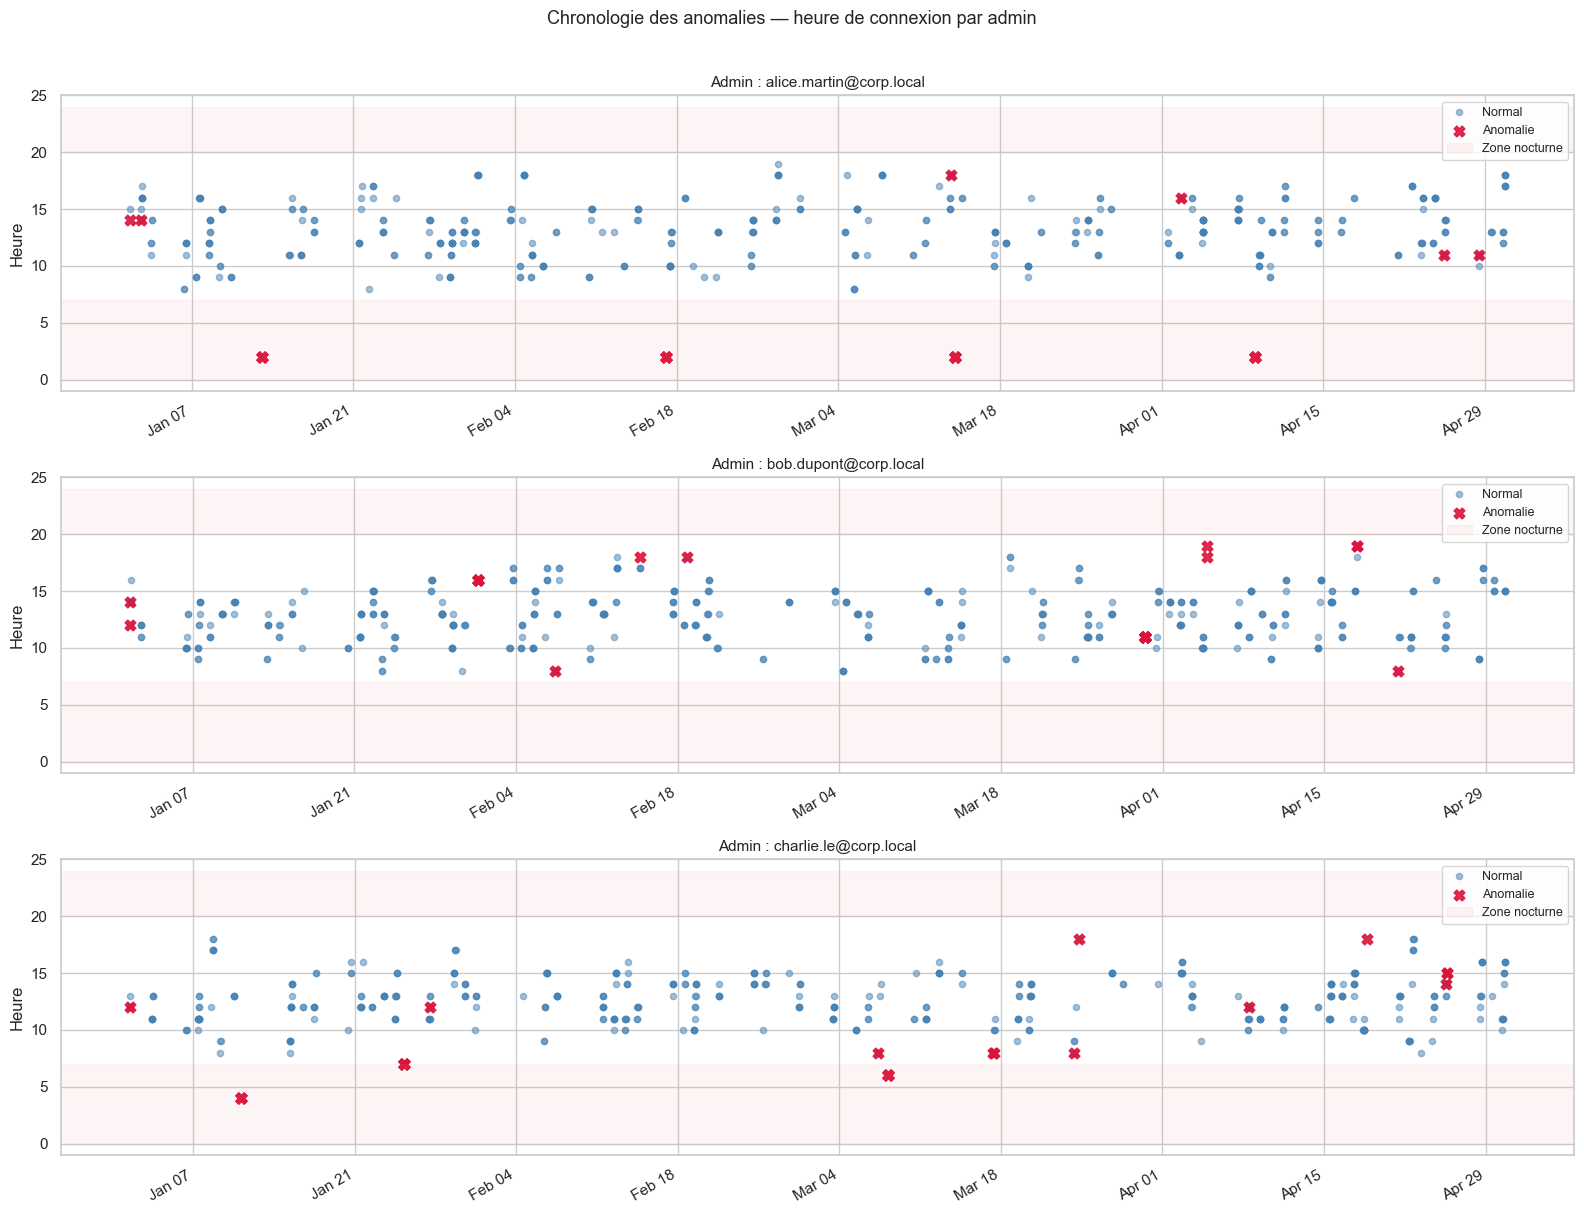
\includegraphics[width=0.98\textwidth]{images/Chronologie des anomalies par admin.png}
	
	\caption{Chronologie des événements administrateur avec points normaux et anomalies détectées. Objectif: vérifier visuellement la cohérence temporelle des alertes par rapport aux habitudes de connexion de chaque administrateur.}
	\label{fig:chronologie_anomalies_admin}
\end{figure}

Lecture: les marqueurs anormaux situés en dehors des plages horaires habituelles (nuit/week-end) sont priorisés pour investigation.

\subsubsection{Heatmap: Score d'anomalie par (jour, heure)}

\begin{figure}[H]
	\centering
		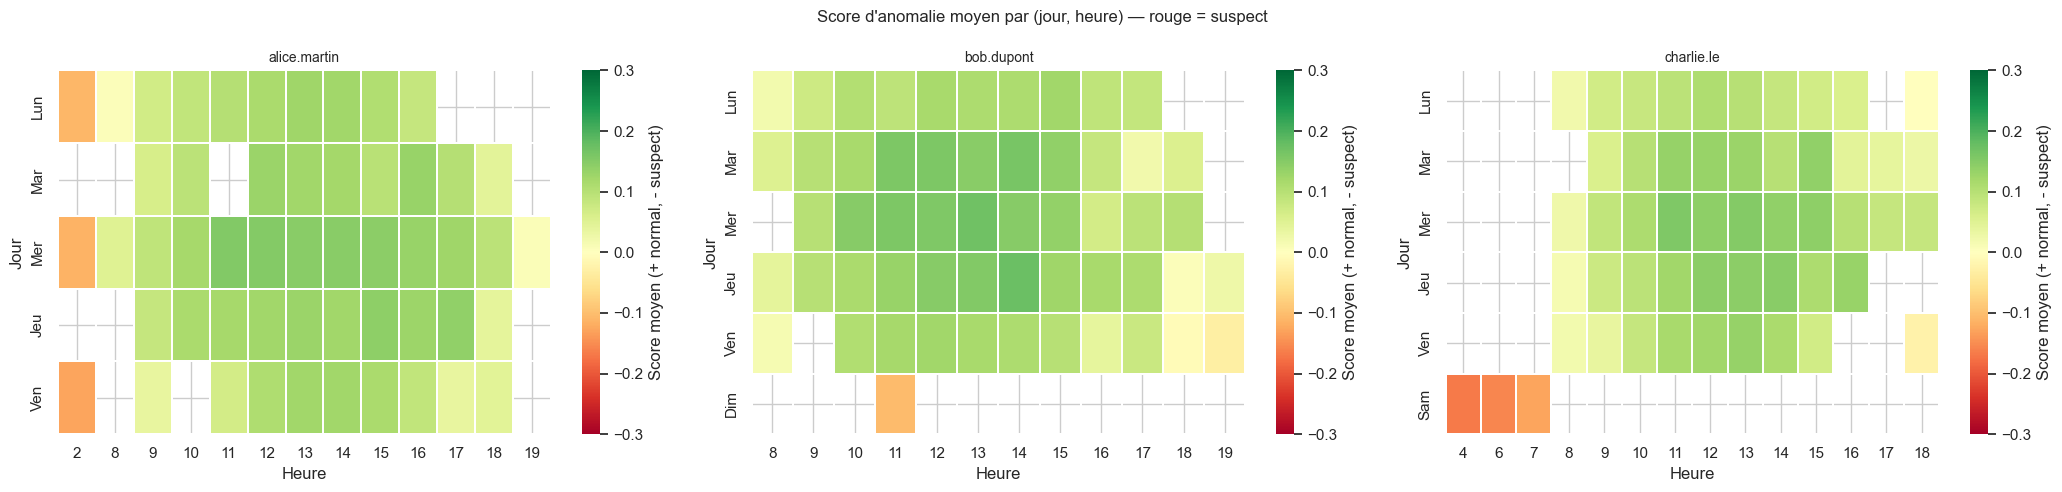
\includegraphics[width=0.98\textwidth]{images/Heatmapscoredanomaliemoyenparheure et jour de la semaine.png}
	
	\caption{Heatmap du score d'anomalie moyen par jour et par heure. Objectif: identifier les zones temporelles à risque où le comportement administrateur s'écarte du profil habituel.}
	\label{fig:heatmap_score_anomalie_admin}
\end{figure}

Lecture: les cellules rouges indiquent des créneaux atypiques et servent à orienter le réglage des seuils de détection.

\subsubsection{Distribution: Nouvelles IP vs anomalies}

\begin{figure}[H]
	\centering
		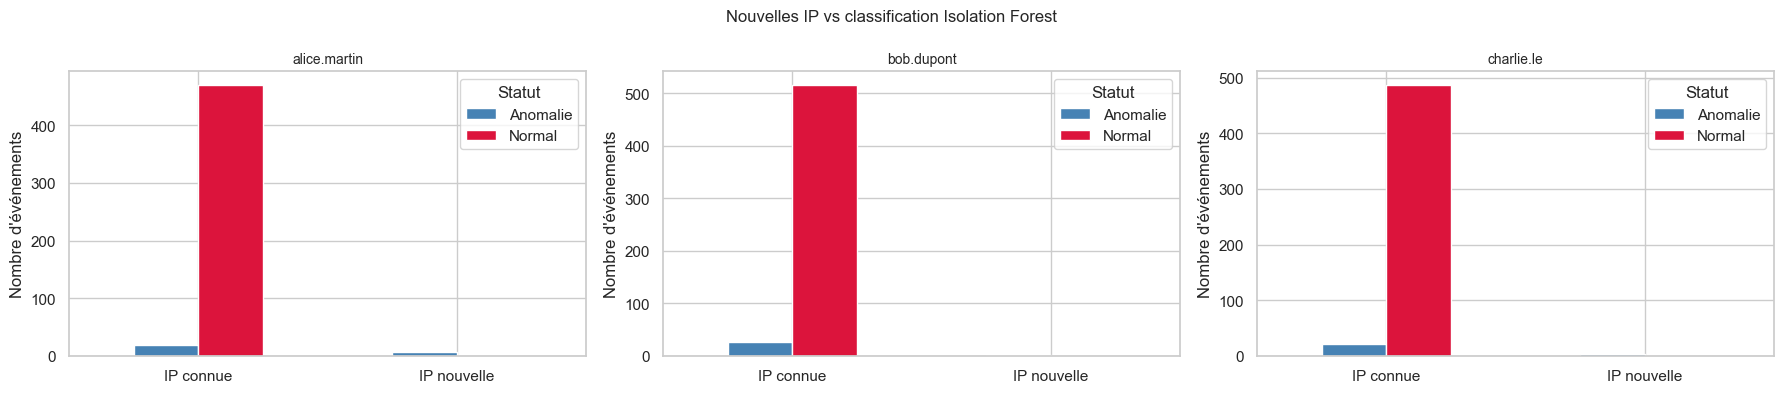
\includegraphics[width=0.98\textwidth]{images/Nouvelles IP vs classification Isolation Forest.png}
	
	\caption{Comparaison entre événements provenant d'IP connues et d'IP nouvelles, selon la classe Normal/Anomalie. Objectif: mesurer la contribution de la nouveauté réseau au risque détecté.}
	\label{fig:nouvelles_ip_vs_anomalies}
\end{figure}

Lecture: une proportion élevée d'anomalies sur IP nouvelles valide la pertinence de la feature \texttt{is\_new\_ip\_for\_admin}.

\subsubsection{Détection de rafales d'approbations}

\begin{figure}[H]
	\centering
		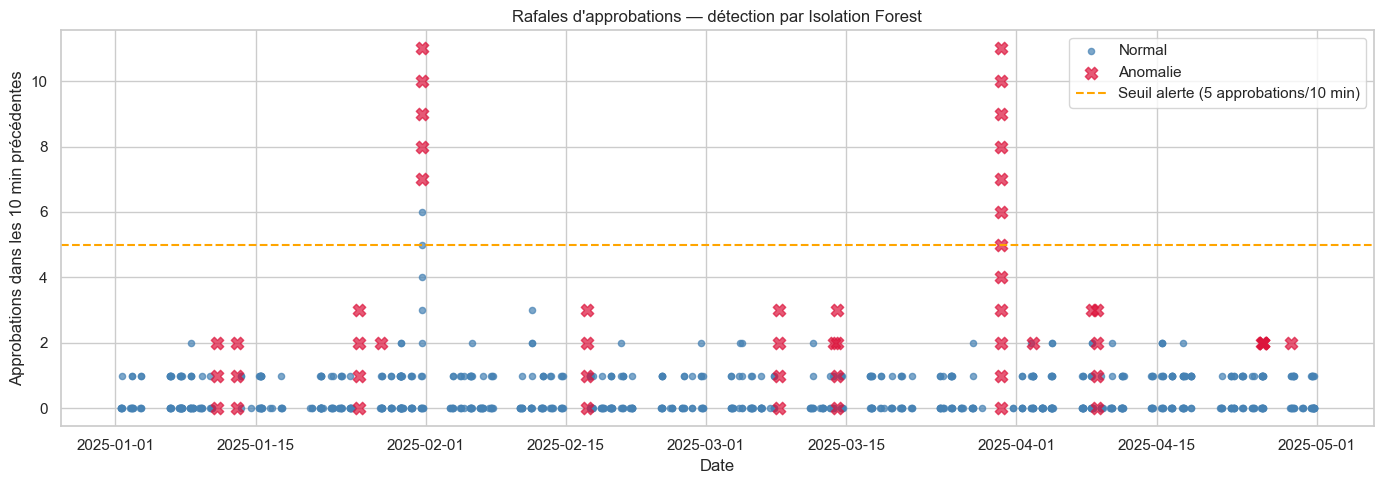
\includegraphics[width=0.98\textwidth]{images/Rafales approbations — détection par Isolation Forest.png}
	
	\caption{Détection des rafales d'approbations sur fenêtre glissante de 10 minutes. Objectif: distinguer l'activité opérationnelle normale des pics d'approbation potentiellement malveillants.}
	\label{fig:rafales_approbations_isolation_forest}
\end{figure}

Lecture: les points anormaux au-dessus du seuil opérationnel (5 approbations/10 min) déclenchent une alerte prioritaire.


\section{Intégration dans le workflow d'approbation JIT}

\subsection{Étape supplémentaire: Vérification d'approbateur}

Le moteur JIT applique maintenant une étape intermédiaire avant validation:

\begin{enumerate}
	\item Utilisateur demande accès $\rightarrow$ état \texttt{pending}.
	
	\item Système sélectionne un approbateur compatible.
	
	\item Moteur de détection d'anomalies évalue l'approbateur en temps réel:
	\begin{itemize}
		\item Si score d'anomalie $> 0.8$: l'approbateur est lui-même suspect. La demande est escaladée à un niveau supérieur ou rejetée.
		\item Si $0.6 < $ score $\leq 0.8$: Approbation possible, mais avec alertes SIEM amplifiées et audit renforcé.
		\item Si score $\leq 0.6$: Approbation autorisée normalement.
	\end{itemize}
	
	\item Approbateur approuve (ou refuse) normalement.
	
	\item Moteur JIT active l'accès et enregistre l'approbateur +  score d'anomalie pour audit ultérieur.
\end{enumerate}

\subsection{Tableau de bord de monitoring}

Le tableau de bord de sécurité affiche:

\begin{table}[h]
\centering
\begin{tabularx}{\textwidth}{|l|l|l|p{5cm}|}
\hline
\textbf{Admin} & \textbf{Score Anomalie (7j)} & \textbf{État} & \textbf{Action} \\
\hline
alice.martin@corp.local & 0.15 & ✓ Normal & - \\
\hline
bob.dupont@corp.local & 0.65 & ⚠ Borderline & Enquête suggérée \\
\hline
charlie.le@corp.local & 0.92 & ✗ Anomalie & Compte suspendu, escalade de sécurité \\
\hline
\end{tabularx}
\caption{Exemple de tableau de bord SOC pour le suivi des comptes privilégiés. Objectif: prioriser la réponse sécurité selon le score d'anomalie et le niveau de risque associé.}
\label{tab:dashboard_anomalies_admin}
\end{table}

\section{Cas d'usage et scénarios}

\subsection{Scénario 1: Compte compromis détecté}

\begin{itemize}
	\item Attaquant gagne accès au compte d'admin Bob via phishing.
	\item Entre 2h-4h du matin (heure attaquant en Asie), lance 30 demandes d'accès en rafale.
	\item Isolation Forest détecte: score anomalie de Bob passe de 0.2 à 0.85 en une nuit.
	\item Alerte SIEM: "Anomalie détectée - Admin Bob - Accès hors horaires habituels".
	\item Équipe sécurité reçoit notification. Enquête: IP de l'attaquant tracée, compte Bob forcé en déconnexion, MFA reconfigurée.
	\item Dommage limité: accès JIT n'a pu être approuvé que 3 fois avant la détection.
\end{itemize}

\subsection{Scénario 2: Privilèges escaladés abusivement}

\begin{itemize}
	\item Admin Alice (rôle standard) tente soudain d'approuver accès pour machines "critiques" (en-dehors de sa portée).
	\item Moteur JIT refuse l'approbation (contrôle RBAC); Isolation Forest marque la tentative comme anomalie.
	\item Alerte: "Escalade de privilèges tentée par Alice".
	\item Enquête révèle qu'Alice a un script malveillant qui tente d'élargir ses permissions.
\end{itemize}

\subsection{Scénario 3: Comportement acceptable mais inhabituel}

\begin{itemize}
	\item Admin Charlie travaille habituellement 9h-17h.
	\item Projet urgent survient; travail nocturne (22h-6h) pendant 5 jours.
	\item Isolation Forest détecte anomalie (score 0.72).
	\item Équipe sécurité valide le contexte auprès de Charlie: Projet X, justification acceptable.
	\item Faux positif reconnu; seuil affiné ou exception documentée.
\end{itemize}

\section{Ajustement et tuning du modèle}

\subsection{Paramètre \texttt{contamination}}

Le paramètre \texttt{contamination} définit le pourcentage d'observations attendues comme anomalies.
Il influence directement la sensibilité du modèle:

\begin{itemize}
	\item \textbf{contamination = 0.02}: Très strict. Suppose 2\% d'anomalies. Peu d'alertes, risque de faux négatifs (manquer les attaques).
	
	\item \textbf{contamination = 0.05}: Recommandé pour PME. Suppose 5\% d'anomalies. Équilibre sensibilité/faux positifs.
	
	\item \textbf{contamination = 0.10}: Permissif. Suppose 10\% d'anomalies. Plus d'alertes, meilleure couverture.
	
	\item \textbf{contamination = 0.20}: Très sensible. Suppose 20\% d'anomalies. Beaucoup de faux positifs.
\end{itemize}

Ajustement recommandé selon contexte:
\begin{itemize}
	\item \textbf{PME sans historique incident}: contamination = 0.05.
	\item \textbf{PME avec quelques incidents}: contamination = 0.05–0.10.
	\item \textbf{Secteur finance/santé/critique}: contamination = 0.02–0.05 (très strict).
\end{itemize}

\subsection{Fenêtre temporelle d'apprentissage}

Le modèle s'entraîne sur des données historiques. Le choix de la fenêtre affecte l'adaptabilité:

\begin{itemize}
	\item \textbf{7 jours}: Capture variations semaine-type. Rapide, réactif aux changements. \textbf{Recommandé au démarrage}.
	
	\item \textbf{14 jours}: Captures 2 semaines = fériés, projets courts. Meilleur équilibre.
	
	\item \textbf{30 jours}: Captures variations mensuelles, congés. Modèle plus stable mais lent à s'adapter aux changements.
	
	\item \textbf{90 jours}: Captures saisonnalité. Très stable mais peu réactif; risque d'oublier nouvelles règles.
\end{itemize}

Recommandation: Démarrer avec 7-14 jours, évaluer faux positifs/négatifs après 2-3 semaines, allonger si stabilité insuffisante.

\subsection{Seuil d'alerte}

Le score d'anomalie varie de 0 (normal) à 1 (fortement anormal). Le seuil détermine quand déclencher une alerte:

\begin{itemize}
	\item \textbf{Seuil $t = 0.80$}: Très strict. Seules les anomalies fortes ($A(x) > 0.80$) déclenchent alerte.
	
	\item \textbf{Seuil $t = 0.70$}: Équilibré (recommandé). Entre normal et attention.
	
	\item \textbf{Seuil $t = 0.60$}: Sensible. Capture anomalies moyennes aussi.
	
	\item \textbf{Seuil $t = 0.50$}: Très sensible. Tout ce qui s'écarte du "très normal" trigger alerte.
\end{itemize}

À tester et affiner en fonction du volume d'alertes et faux positifs observés.

\subsubsection{Approche progressive}

\begin{enumerate}
	\item Démarrer avec seuil 0.75 (très strict).
	\item Observer pendant 1 mois.
	\item Si trop peu d'alertes: réduire à 0.70 ou 0.60.
	\item Si trop de faux positifs: augmenter à 0.80.
	\item Documenter les seuils ajustés et les raisons.
\end{enumerate}

\section{Limitations et considérations}

\subsection{Problème du cold start}

Lors du démarrage du système, \textbf{toute IP est "nouvelle"} pour chaque administrateur, car aucun historique 30-jours n'existe.

\textbf{Mitigation}:
\begin{itemize}
	\item Réduire la période lookback lors des premières semaines (ex: 5 jours au lieu de 30).
	\item Ignorer ou pondérer moins fortement \texttt{is\_new\_ip\_for\_admin} pendant les 2 premières semaines.
	\item Laisser tourner le système en mode "debug" (alertes non-bloquantes) pendant 30 jours avant production.
\end{itemize}

\subsection{Faux positifs: Comportements légitimes inhabituels}

Isolation Forest peut flaguer comme anormal:
\begin{itemize}
	\item \textbf{Projet d'urgence}: Travail nocturne nécessaire (est marqué "is\_night"=1 $\Rightarrow$ anomalie).
	\item \textbf{Télétravail soudain}: IP change (est marqué "is\_new\_ip"=1 $\Rightarrow$ anomalie).
	\item \textbf{Changement de rôle}: Nouvel admin hérite habits différents (débute zéro historique).
	\item \textbf{Congé suivi de surcharge}: Pic d'activités post-vacances (approvals\_last\_10min élevé).
\end{itemize}

\textbf{Mitigation}:
\begin{itemize}
	\item Documenter exceptions approuvées (ex: "Alice = télétravail définitif depuis 15/03/2025").
	\item Implémenter système de \textit{whitelist} d'IPs ou heures spéciales pour chaque admin.
	\item Utiliser 2 seuils: $t_{\text{strict}}=0.80$ (alerte immédiate) et $t_{\text{warning}}=0.60$ (inspection manuelle).
	\item Créer un tableau de bord pour SecurityOps: réviser les 10 principales anomalies par mois, puis valider ou rejeter.
\end{itemize}

\subsection{Concept Drift (dérive de concept)}

Le comportement normal d'un admin peut se modifier graduellement:
\begin{itemize}
	\item Télétravail permanent (IP change).
	\item Promotion vers rôle avec horaires décalés (heure change).
	\item Changements saisonniers (moins d'approbations en été).
\end{itemize}

Ce qui était anomalie hier devient normal aujourd'hui.

\textbf{Mitigation}:
\begin{itemize}
	\item \textbf{Réentraînement régulier}: réentraîner le modèle de manière hebdomadaire ou mensuelle.
	\item \textbf{Fenêtre glissante}: Utiliser "rolling window" des 30 derniers jours (pas figé).
	\item \textbf{Feedback loop}: Si alerte marquée "faux positif" par SecurityOps, intégrer dans données futures.
	\item \textbf{Monitoring du drift}: Tracker "score moyen par admin" — si hausse progressive = concept drift détecté.
\end{itemize}

\subsection{Comptes de service et bots}

Les comptes de service (intégrations, jobs cron, robots) ont des patterns totalement différents:
\begin{itemize}
	\item Connexions à \textbf{heures fixes} (00:05, 12:15 précisément).
	\item \textbf{Très fréquentes} (1000+ par jour) $\Rightarrow$ \texttt{approvals\_last\_10min} toujours élevé.
	\item De \textbf{mêmes IPs} (pas d'IP nouvelles).
	\item Pas de concept "jour/nuit" ou "week-end".
\end{itemize}

Entraîner Isolation Forest sur ces comptes produirait alertes inutiles.

\textbf{Mitigation}:
\begin{itemize}
	\item Créer \textbf{modèles séparés}: un pour "admins humains", un pour "service accounts".
	\item Ou exclure entièrement service accounts de cette détection (ils relèvent d'autres contrôles).
	\item Tagguer les comptes en fonction de type (attribut "account\_type" = "human" ou "bot").
\end{itemize}

\subsection{Données manquantes ou corrompues}

Si logs Wazuh Indexer sont incomplets (dépôt échoué, agent down), features seront biaisées.

\textbf{Mitigation}:
\begin{itemize}
	\item Checker santé agents Wazuh avant extraction.
	\item Ignorer jours avec < 50\% data pour admin (données insuffisantes).
	\item Implémenter alerte "données manquantes pour admin X" $\Rightarrow$ détection temporairement désactivée pour X.
\end{itemize}

\subsection{Respect de la vie privée (RGPD)}

Collecter et analyser logs d'administrateur soulève questions RGPD:
\begin{itemize}
	\item \textbf{Légal}: Les administrateurs doivent consentir ou avoir justification légitime (sécurité).
	\item \textbf{Transparence}: Communication claire que surveillance effectuée.
	\item \textbf{Rétention}: Combien de temps conserver les logs? (Recommandation: 90 jours max).
	\item \textbf{Accès}: Qui peut voir les alertes? (responsables sécurité).
\end{itemize}

\textbf{Mitigation}:
\begin{itemize}
	\item Documenter base légale dans politique de sécurité.
	\item Chiffrer logs et alertes en transit/repos.
	\item Implémenter contrôle d'accès (RBAC) sur dashboard anomalies.
	\item Archiver et supprimer logs après rétention.
\end{itemize}

\section{Conclusion du chapitre}

La détection d'anomalies appliquée aux administrateurs répond à la question critique \textit{"Qui garde les gardiens?"} 
en mettant en place une \textbf{surveillance comportementale continue basée sur les données réelles} provenant de Wazuh Indexer.

\subsection{Pipeline complet}

Le système fonctionne selon ce processus:

\begin{enumerate}
	\item \textbf{Collecte}: Agents Wazuh sur chaque service (Authentik, moteur JIT, SSH) envoient logs au Wazuh Manager.
	
	\item \textbf{Centralisation}: Wazuh Indexer (OpenSearch/Elasticsearch) centralise et indexe tous les logs.
	
	\item \textbf{Extraction}: Script Python récupère les logs administrateur via requêtes API Wazuh (dernières 7-30 jours).
	
	\item \textbf{Feature engineering}: Calcul de 8 features comportementales (heure, jour, IP nouvelle, rafales, etc.).
	
	\item \textbf{Détection ML}: Isolation Forest entraîné par admin détecte anomalies (score 0-1).
	
	\item \textbf{Alertes}: Scores > 0.60-0.75 génèrent custom alerts dans Wazuh + notifications SecurityOps.
	
	\item \textbf{Décision JIT}: Avant d'approuver une demande d'accès, le moteur JIT consulte le score d'anomalie 
	du demandeur $\Rightarrow$ peut refuser ou escalader si approbateur lui-même suspect.
	
	\item \textbf{Audit}: Tous les scores d'anomalie sont loggés pour audit/historique (traçabilité complète).
	
	\item \textbf{Feedback}: SecurityOps valide alertes; faux positifs $\Rightarrow$ raffinement modèle.
\end{enumerate}

\subsection{Avantages de cette approche}

\begin{itemize}
	\item \textbf{Données réelles}: Basé sur logs vrais provenant de Wazuh, pas synthétiques.
	
	\item \textbf{Non-supervisé}: Pas besoin d'étiqueter "normal" vs. "anormal" manuellement.
	
	\item \textbf{Modèles individuels}: Un profil par admin $\Rightarrow$ détecte écarts personnels.
	
	\item \textbf{Interprétable}: Isolation Forest fournit features explicatives (pourquoi flagué).
	
	\item \textbf{Léger}: Exécutable sur ressources limitées (cron job sur serveur sécurité).
	
	\item \textbf{Zero Trust}: Couvre la boucle complète: même les administrateurs restent sous surveillance.
\end{itemize}

\subsection{Métriques de succès}

Après déploiement, tracker:

\begin{itemize}
	\item \textbf{Taux de détection}: Combien d'anomalies réelles (comptes compromis) détectées avant dommage?
	
	\item \textbf{Faux positifs}: Combien d'alertes invalides par mois? (Cible: < 10\%).
	
	\item \textbf{MTTR (Mean Time To Response)}: Temps entre alerte et action SecurityOps (Cible: < 30 min).
	
	\item \textbf{Stabilité modèle}: Score moyen/écart-type par admin stable ou dérives?
	
	\item \textbf{Couverture}: Quel \% d'admins ont au moins 10 logs/jour pour entraînement fiable?
\end{itemize}

\subsection{Perspectives d'amélioration}

\begin{enumerate}
	\item \textbf{Enrichissement IP}: Ajouter résolution GeoIP (pays, ASN) pour détecter changements géo impossibles.
	
	\item \textbf{Corrélation multi-événements}: Lier anomalies d'admin à alertes parallèles (ex: approbation anormale + tentative privilège escalade sur machine).
	
	\item \textbf{Modèles supervisés hybrides}: Si suffisante données labelisées, combiner Isolation Forest + modèles supervisés (RandomForest, XGBoost).
	
	\item \textbf{Apprentissage par renforcement}: Système qui apprend du feedback SecurityOps en temps réel.
	
	\item \textbf{Graphes de comportement}: Représenter les admins et leurs interactions (qui approuve qui, qui peut accéder où) en tant que graphe; détection d'anomalies sur graphes (Graph Neural Networks).
\end{enumerate}

\subsection{Résumé}

En combinant collecte centralisée (Wazuh), ingénierie de features comportementales, Isolation Forest ML, 
et intégration JIT, nous établissons un système robuste de détection des anomalies administrateur. 

Cette approche transforme la gestion des administrateurs d'une \textit{position de confiance implicite} 
à un modèle \textit{de vérification continue et automatisée}, aligné pleinement avec l'esprit \textbf{Zero Trust} du projet.